%-----------------------Homework------------------------------------
%-------------------Arman Shokrollahi---------------------------------
%---------------------Introduction to Electrical and Electronic Engineering-------------------------------

\documentclass[a4 paper]{article}
% Set target color model to RGB
\usepackage[inner=1.5cm,outer=1.5cm,top=2.5cm,bottom=2.5cm]{geometry}
\usepackage{setspace}
\usepackage[rgb]{xcolor}
\usepackage{verbatim}
\usepackage{amsgen,amsmath,amstext,amsbsy,amsopn,tikz,amssymb,tkz-linknodes}
\usepackage{fancyhdr}
\usepackage[colorlinks=true, urlcolor=blue,  linkcolor=blue, citecolor=blue]{hyperref}
\usepackage[colorinlistoftodos]{todonotes}
\usepackage{rotating}
\usepackage{multirow}
\usepackage{graphicx}
\usepackage{paracol}
\usepackage{color}
\newcommand{\blue}[1]{\textcolor{blue}{#1}}
\newcommand{\red}[1]{\textcolor{red}{#1}}
\newcommand{\green}[1]{\textcolor{green}{#1}}
\newcommand{\yellow}[1]{\textcolor{yellow}{#1}}
\newcommand{\orange}[1]{\textcolor{orange}{#1}}
\newcommand{\violet}[1]{\textcolor{violet}{#1}}

%\usetikzlibrary{through,backgrounds}
\hypersetup{%
pdfauthor={Nan Meng},%
pdftitle={Notes},%
pdfkeywords={Tikz,latex,bootstrap,uncertaintes},%
pdfcreator={PDFLaTeX},%
pdfproducer={PDFLaTeX},%
}
%\usetikzlibrary{shadows}
\usepackage[francais]{babel}
\usepackage{booktabs}
\newcommand{\ra}[1]{\renewcommand{\arraystretch}{#1}}

      \newtheorem{thm}{Theorem}[section]
      \newtheorem{prop}[thm]{Proposition}
      \newtheorem{lem}[thm]{Lemma}
      \newtheorem{cor}[thm]{Corollary}
      \newtheorem{defn}[thm]{Definition}
      \newtheorem{rem}[thm]{Remark}
      \numberwithin{equation}{section}

\newcommand{\homework}[6]{
   \pagestyle{myheadings}
   \thispagestyle{plain}
   \newpage
   \setcounter{page}{1}
   \noindent
   \begin{center}
   \framebox{
      \vbox{\vspace{2mm}
    \hbox to 6.28in { {\bf ENGG1203:~Introduction to Electrical and Electronic Engineering \hfill} }
       \vspace{6mm}
       \hbox to 6.28in { {\Large \hfill #1 (#2)  \hfill} }
       \vspace{6mm}
       \hbox to 6.28in { {\it Instructor: #3 \hfill TA: #5} }
       %\hbox to 6.28in { {\it TA: #4  \hfill #6}}
      \vspace{2mm}}
   }
   \end{center}
   \markboth{#5 -- #1}{#5 -- #1}
   \vspace*{4mm}
}

\newcommand{\bbF}{\mathbb{F}}
\newcommand{\bbX}{\mathbb{X}}
\newcommand{\bI}{\mathbf{I}}
\newcommand{\bX}{\mathbf{X}}
\newcommand{\bY}{\mathbf{Y}}
\newcommand{\bepsilon}{\boldsymbol{\epsilon}}
\newcommand{\balpha}{\boldsymbol{\alpha}}
\newcommand{\bbeta}{\boldsymbol{\beta}}
\newcommand{\0}{\mathbf{0}}

\begin{document}
\homework{\bf Circuits}{ENGG1203}{Edmund Y.Lam}{}{Nan Meng}{}

% {\begin{tikzpicture}[outline/.style={draw=#1,thick,fill=#1!50}]
% \node [outline=red] at (0,1) {\bf Problem 1};
% \end{tikzpicture}}

\section{Basics}

We use a simple model as a starting point to discuss electronic circuits, which is shown on Figure \ref{fundamental}.

\begin{figure}[!ht]
  \caption{Fundamental circuit model}
  \label{fundamental}
  \centering
  \includegraphics[width=0.5\textwidth]{./images/introduction}
\end{figure}

\vskip 1em
A basic circuit is made up of a \underline{source} which provides voltage across its terminals, denoted by $V_s$. and a \underline{load} connected to the source which presents a resistance $R_L$ to the current $i$ flowing as indicated around a closed loop.



% --------------------------------------------------------
% --------------------------------------------------------


\subsection{Current}
The current $i$ results from the stream of electric charge around the closed loop shown on Figure 1. The mathematic definition is equal to the amount of charge, $Q$, passing through a cross-section per second and it can be expressed as
\begin{equation}
i = \frac{dQ}{dt} 
\end{equation}
The unit of charge is Coulomb. One Coulomb is equivalent to $6.24 \times 10^{18}$ electrons.
The unit of current is ampere, {\bf A}. 1 Ampere = 1 Coulomb/sec.
 
\subsubsection{Ideal DC Current Source}
The current source is a device that can provide a certain amount of current to a circuit. The symbol for a DC current source and the i / v characteristic curve of an ideal current source are shown on Figure \ref{currentsource}.
\begin{figure}[!ht]
  \caption{Ideal DC Current Source}
  \label{currentsource}
  \centering
  \includegraphics[width=0.09\textwidth]{./images/circuit1/current1}
\end{figure}


% --------------------------------------------------------
% --------------------------------------------------------


\subsection{Voltage}
Moving electrons along a conductor requires some amount of work that must be somehow supplied by an electromotive force provided by a battery or similar device. The electromotive force is the potential difference(voltage) between two points or across a component in circuit. The mathematical definition of voltage is given by
\begin{equation}
v = \frac{dW}{dQ} 
\end{equation}

where work(W) is measured in Joules and charge(Q) in Coulombs.
Basically, the voltage is measured in volts(V) and $1 volt = 1 \frac{Joule}{Coulomb} = 1 \frac{Newton \ meter}{Ampere \ second}$

\subsubsection{Ideal DC Voltage Source}
The voltage provided by a voltage source(usually battery) is constant in time and thus it is called DC voltage. In its ideal implementation the battery provides a specific voltage at all times and for all loads.
The symbols of an ideal DC voltage source are shown as follows:

\begin{figure}[!ht]
  \caption{Ideal DC Voltage Source}
  \centering
  \includegraphics[width=0.3\textwidth]{./images/circuit1/VoltageSource}
\end{figure}



% --------------------------------------------------------
% --------------------------------------------------------

\subsection{Ideal resistor}
The ideal resistor is a passive, linear, two-terminal device whose resistance follows Ohm`s law given by,
\begin{equation}
v = iR,
\end{equation}
which states that the voltage across an element is directly proportional to the current flowing through the element. The constant of proportionality is the resistance R provided by the element. The resistance is measured in Ohms, $\Omega$, and
\begin{equation}
1 \Omega = 1 \frac{V}{A},
\end{equation}
the symbol for a resistor is,

\begin{figure}[!ht]
  \caption{Ideal resistor}
  \centering
  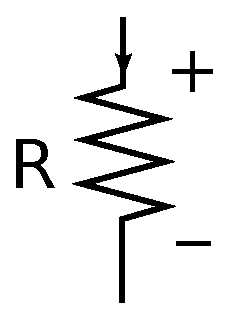
\includegraphics[width=0.1\textwidth]{./images/circuit1/resistor}
\end{figure}



\subsection{Resistor Color Code}
The colored painted bands produce a system of identification generally known as a {\bf Resistors Color Code}.
The resistor color code markings are always read one band at a time starting from the left to the right, with the larger width tolerance band oriented to the right side indicating its tolerance. By matching the color of the first band with its associated number in the digit column of the color chart below, the first digit is identified and this represents the first digit of the resistance value.

Again, by matching the color of the second band with its associated number in the digit column of the color chart, we get the second digit of the resistance value and so on. Then the resistor color code is read from left to right as illustrated below

\begin{figure}[!ht]
  \caption{Resistor Color Code}
  \centering
  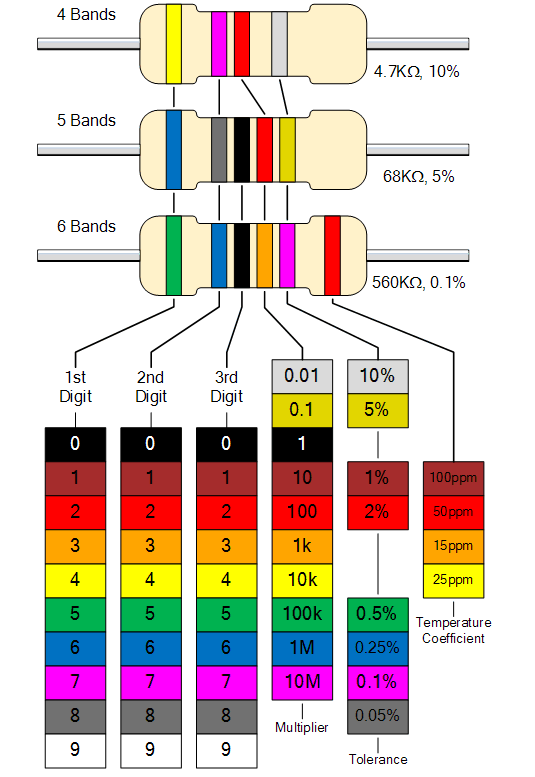
\includegraphics[width=0.5\textwidth]{./images/ColourCode1}
\end{figure}

\vspace{8 mm}

\begin{figure}[!ht]
  \caption{Color Code Table}
  \centering
  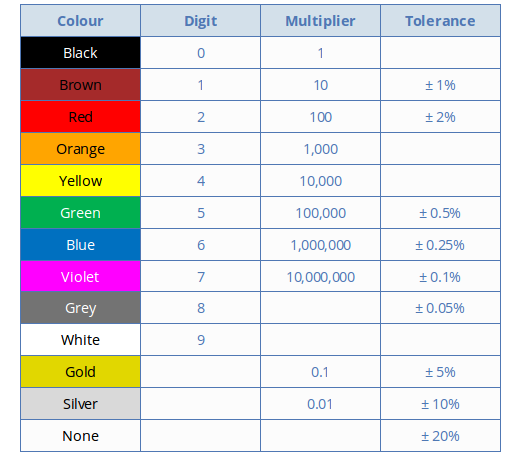
\includegraphics[width=0.5\textwidth]{./images/ColourCode2}
\end{figure}
For example, a resistor has the following colored markings: \newline
\centerline{\yellow{Yellow} \violet{Violet} \red{Red} = \yellow{4} \violet{7} \red{2} = \yellow{4} \violet{7}$\times$ \red{$10^2$} = 4700$\Omega$ or 4k7.
}

\subsection{Power}
When current flows through a resistor, energy is irreversibly lost(or we say dissipated) in overcoming the resistance. The dissipated power shows up as heat most of the time. The mathematical definition of power is the rate at which energy is delivered. It can be expressed as
\begin{equation}
P = \frac{dW}{dt},
\end{equation}
The units for power are $Joules/sec$ or Watts, $W$. ($1 Joules/sec = 1 W$)
Power can be related to voltage and current by rewriting Eq.(1.5) as, 

\begin{equation}
P = \frac{dW}{dt} = \frac{dW}{dQ}\frac{dQ}{dt}=vi,
\end{equation}

Then substitute Ohm's law in Eq.(1.6), we will get the power dissipated in a resistor of resistance R is a quadratic function of either $i$ or $v$ and they can be expressed by

\begin{equation}
P = i^2R \quad or \quad P = \frac{v^2}{R}
\end{equation}
Power rating is a fundamental constraint of resistors and electronic devices in general. The power rating is referred to the maximum power that the device can dissipate without adversely affecting its operation. When the power rating is exceeded, the resistor overheats and it is destroyed by burning up. 




% --------------------------------------------------------------
% --------------------------------------------------------------

\section{Kirchhoff's Laws}
Kirchhoff's laws also known as Kirchhoff's Current Law (KCL) and Kirchhoff's Voltage Law (KVL) are based respectively on the conservation of charge and the conservation of energy and are derived from Maxwell's equations. They along with Ohm's law present the fundamental tools for circuit analysis.
\subsection{Kirchhoff's Current Law}
The current flowing out of any node in a circuit
must be equal to the current flowing into the node. It is expressed mathematically as
\begin{equation}
\sum_{n=1}^{N}i_n=0
\end{equation}

where N is the number of branches that are connected to the node. 
\subsection{Kirchhoff's Voltage Law}
The algebraic sum of voltages around a closed loop is zero. It is expressed mathematically as
\begin{equation}
\sum_{n=1}^{N}v_n=0
\end{equation}

where N is the number of voltages in the loop. The number of voltages is equal to the number of elements encountered as we go around the loop.

\vspace{60 mm}
Next we will solve for the circuit shown on Figure 7

\begin{figure}[ht!]
  \caption{Example resistive circuit}
  \centering
  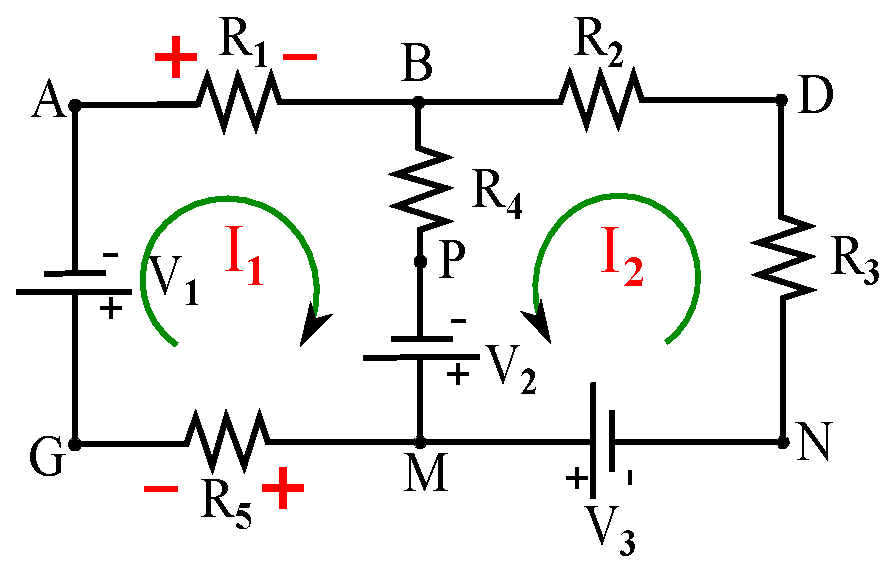
\includegraphics[width=0.5\textwidth]{./images/circuit1/circuit5_1}
\end{figure}
\blue{\centerline{\bf $R_1 = 80\Omega$, $R_2 = 10\Omega$, $R_3 = 20\Omega$, $R_4 = 90\Omega$, $R_5 = 100\Omega$, $V_1 = 12V$, $V_2 = 24V$, $V_3 = 36V$}}

\vspace{8 mm}
Apply Kirchhoff's laws.

\begin{itemize} \itemsep2pt \parskip0pt \parsep0pt
  \item[$\bullet$] Start with the nodes.
  \begin{enumerate} \itemsep2pt \parskip0pt \parsep0pt
  \item The middle node P is already accounted for since we assigned the current above and below it the same value, I$_1$.  This is just Kirchhoff's current law which says that the current going into a node is equal to that going out. 
  \item The bottom and top nodes B and M are exactly the same and KCL for them is:
  \item[] \hspace{6 cm}{$I - I_1 + I_2 = 0$}\newline
  since at node B, current $I$ and $I_2$ flow in the node B and $I_1$ flows out the node B.
  \end{enumerate}
  \item[$\bullet$] Next let's apply KVL to the three loops
  \begin{enumerate} \itemsep1pt \parskip0pt \parsep0pt
    \item {\bf Loop 1($I_1$ loop):} voltage source $V_1$, $V_2$ and resistors $R_1$, $R_4$, $R_5$ \newline\newline
    \centerline{$V_1 + I_1R_1 + (I_1+I_2)R_4 - V_2 + I_1R_5 = 0$}\newline
    \item[] \hspace{56 mm}$\Rightarrow 12 + 80I_1 + 90I_1 + 90I_2 - 24 + 100I_1 = 0$
    \newline
    \item[] \hspace{56 mm}$\Rightarrow 270I_1 + 90I_2 = 12$
    \newline

    \item {\bf Loop 2($I_2$ loop):} voltage source $V_2$, $V_3$ and resistors $R_2$, $R_3$, $R_4$ \newline\newline
    \centerline{$V_3 + I_2R_3 + I_2R_2 + (I_1 + I_2)R_4 -V_2 = 0$}
    \newline
    \item[] \hspace{56 mm}$\Rightarrow 36 + 20I_2 + 10I_2 + 90I_1 + 90I_2- 24 = 0$ \newline
    \item[] \hspace{56 mm}$\Rightarrow 90I_1 + 120I_2 = -12$
    \newline
  
  \end{enumerate}
  \item[$\bullet$] Calculate the required parameters using Ohm`s law and relevant formulas.
  \begin{enumerate} \itemsep1pt \parskip0pt \parsep0pt
    \item[] \centerline{$I_1 = \frac{14}{135}A$}
    \item[] \centerline{$I_2 = -\frac{8}{45}A$}
  \end{enumerate}

\end{itemize}








\section{Voltage divider: Series Connection of Resistors}
The voltage divider circuit is the most convenient means of passively stepping down the voltage from a fixed voltage source. 


\begin{figure}[ht!]
  \centering
  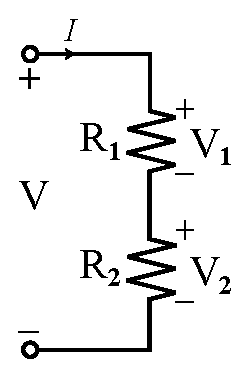
\includegraphics[width=0.15\textwidth]{./images/circuit1/append_end2}
\end{figure}


\begin{itemize} \itemsep1pt \parskip0pt \parsep0pt 
  \item[] \hspace{6.6 cm}{$I=\frac{V}{R_1 + R_2}$}
  \item[] \hspace{6.6 cm}$V_1 = R_1I = \frac{R_1}{R_1 + R_2}V$
  \item[] \hspace{6.6 cm}$V_2 = R_2I = \frac{R_2}{R_1 + R_2}V$
\end{itemize}

By considering a circuit where we are using N resistors connected in series, we can show that the equivalent resistance is the sum of the resistances.

\begin{equation}
R_{eq} = \sum_{n=1}^{N}R_n=R_1+R_2+...+R_N
\end{equation}


\section{Current Divider: Parallel connection of resistors}
The schematic on Figure 8 shows a simple current divider circuit. Here the two resistors $R_1$ and $R_2$ are connected in parallel. Lets determine the current $I_1$ and $I_2$ flowing in the two resistors.

\begin{figure}[ht!]
  \caption{Current Divider}
  \centering
  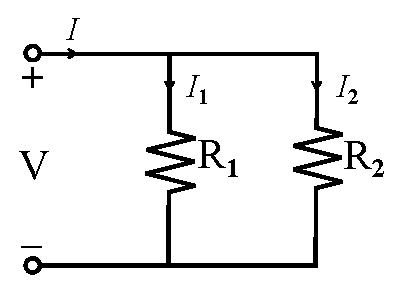
\includegraphics[width=0.3\textwidth]{./images/circuit1/append_end2_2}
\end{figure}
\begin{itemize} \itemsep1pt \parskip0pt \parsep0pt
  \item[] \hspace{6 cm}$V = (R_1 \parallel R_2)I$
  \item[] \hspace{6 cm}$I_1 = \frac{V}{R_1} = \frac{R_1\parallel R_2}{R_1}I = \frac{R_2}{R_1+R_2}I$
  \item[] \hspace{6 cm}$I_2 = \frac{R_1}{R_1 + R_2}I$
\end{itemize}
\vspace{8 mm}

For N resistors connected in parallel the equivalent resistance is 

\begin{equation}
\frac{1}{R_{eq}} = \sum_{n=1}^{N}\frac{1}{R_n}=\frac{1}{R_1}+\frac{1}{R_2}+...+\frac{1}{R_N}
\end{equation}
Note that the equivalent resistance $R_{eq}$ is smaller than the smallest resistance in the parallel arrangement.  

The equivalent conductance of  N resistors connected in parallel is  

\begin{equation}
G_{eq} = \sum_{n=1}^{N}G_n=G_1+G_2+...+G_N
\end{equation}

where $G_n = \frac{1}{R_n}$. The current flowing through resistor $R_n$ is 

\begin{equation}
i_n = i\frac{G_n}{G_{eq}}
\end{equation}

\section{Advanced methods for circuit analysis}
\subsection{Node Method \& Mesh Method}
With the help of Kirchhoff`s laws and Ohm`s law, we can analyze any circuit to determine the currents and voltages. For formal circuit analysis, the challenge is to derive the smallest set of simultaneous equations that completely define the operating characteristics of a circuit.

The following part, we will develop two very powerful methods for analyzing any circuit: The {\bf node method} and the {\bf mesh method}. We will explain the steps to solve the circuit problem shown in Figure 2.











\subsubsection{The Node Method}


Voltage is defined as the potential difference between two points. When we talk about the voltage at a certain point, we imply that the measurement is performed between that point and some other points in the circuit. Usually, this reference point is defined as \red{ground}.

Node method(or node voltage method) is an efficient circuit analysis method based on KCL, KVL, and Ohm's laws. Steps for using node method to analyze circuit are as follows:

\begin{enumerate} \itemsep1pt \parskip0pt \parsep0pt
  \item \blue{Label all the circuit parameters and distinguish the unknown parameters from the known ones.}
  \item \blue{Identify all nodes of the circuit.}
  \item \blue{Choose a reference node(Ground) and assign to it a potential of $0V$. All other voltages in the circuit are measured with respect to the reference node.}
  \item \blue{Label the voltage at all other nodes.}
  \item \blue{Assign and label polarities.}
  \item \blue{Apply KCL at each node and express the branch currents in terms of the node voltages.}
  \item \blue{Solve the resulting simultaneous equations for the node voltages.}
  \item \blue{Obtain the branch currents by Ohm`s law.}
\end{enumerate}

We will use the circuit of Figure 9 for a step by step demonstration of the node method. 

\begin{figure}[ht!]
  \caption{A typical resistive circuit}
  \centering
  \includegraphics[width=0.45\textwidth]{./images/nodemethod_0}
\end{figure}

Figure 10. shows the implementation of steps 1 and 2. We have labeled all elements and identified all relevant nodes in the circuit.  

\begin{figure}[ht!]
  \caption{Circuit with labeled nodes}
  \centering
  \hspace{5 mm}
  \includegraphics[width=0.45\textwidth]{./images/nodemethod_1}
\end{figure}


The third step is to select one of the identified nodes as the reference node. We have four different choices for the assignment. In principle any of these nodes may be selected as 
the reference node. However, some nodes are more useful than others. Useful nodes are the ones which make the problem {\bf easier to understand and solve}. There are a few general guidelines that we need to remember as we make the selection of the reference node. 


\begin{enumerate} \itemsep1pt \parskip0pt \parsep0pt
  \item[$\ast$] \red{A useful reference node is one which should have the largest number of elements connected to it.}
  \item[$\ast$] \red{A useful reference node is one which should be connected to the maximum number of voltage sources.}
\end{enumerate}

In this example the selection of node \blue{{\bf 0}} as the reference node is the best choice. (you could also select node \blue{{\bf 1}} as our reference node.) 

Next, we should label the voltages at the selected nodes. Figure 11 shows the circuit with the labeled nodal voltages. The reference node is assigned voltage 0 Volts indicated by the ground symbol. The remaining node voltages are labeled $V_{S1}$, $V_{S2}$, $V_{S3}$.


\begin{figure}[ht!]
  \caption{Circuit with assigned nodal voltages}
  \centering
  \includegraphics[width=0.5\textwidth]{./images/nodemethod_3}
\end{figure}


For the next step we assign current flow and polarities, see Figure 12.
\begin{figure}[ht!]
  \caption{Example circuit with assigned node voltages and polarities}
  \centering
  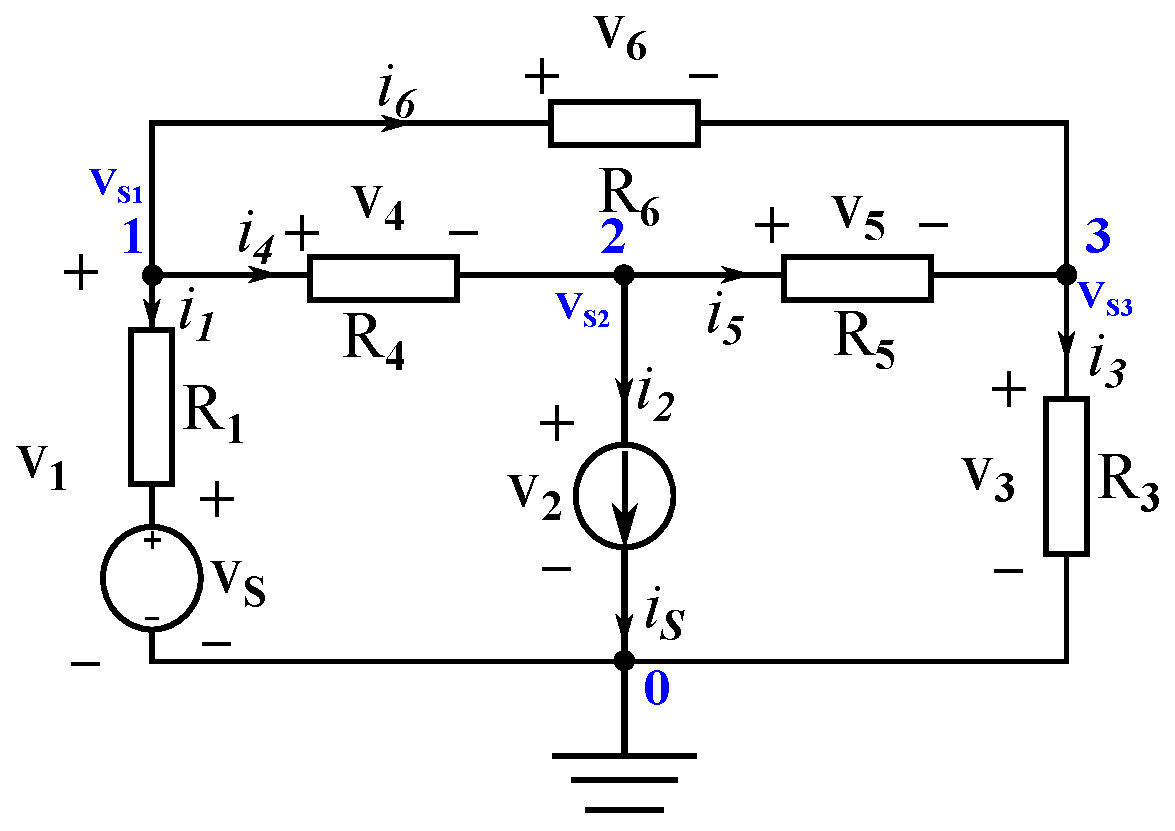
\includegraphics[width=0.5\textwidth]{./images/nodemethod_4}
\end{figure}
The circuit shown on Figure 4 is completely defined now. Once we determine the values for the node voltages $V_{S1}$, $V_{S2}$, $V_{S3}$. we will be able to completely characterize this circuit. So let's go on to calculate the node voltages by applying KCL at the designated nodes. \newline


According to the Ohm's law, the currents $i_1$ to $i_6$ are expressed in terms of the voltages $v_{s1}$, $v_{s2}$, $v_{s3}$ as follows. 
\begin{itemize} \itemsep1pt \parskip0pt \parsep0pt 
  \item[] \hspace{6.6 cm}\begin{equation}i_1 = \frac{v_1-v_s}{R_1}\end{equation}
  \item[] \hspace{6.6 cm}\begin{equation}i_2 = i_s\end{equation}
  \item[] \hspace{6.6 cm}\begin{equation}i_3 = \frac{v_3}{R_3} = \frac{v_{s3}}{R_3}\end{equation}
  \item[] \hspace{6.6 cm}\begin{equation}i_4 = \frac{v_4}{R_4} = \frac{v_{s1}-v_{s2}}{R_4}\end{equation}
  \item[] \hspace{6.6 cm}\begin{equation}i_5 = \frac{v_5}{R_5} = \frac{v_{s2}-v_{s3}}{R_5}\end{equation}
  \item[] \hspace{6.6 cm}\begin{equation}i_6 = \frac{v_6}{R_6} = \frac{v_{s1}-v_{s3}}{R_6}\end{equation}
\end{itemize}

\vspace{8 mm}

KCL at node \blue{{\bf 1}},\blue{{\bf 2}},\blue{{\bf 3}} we will get:


\begin{itemize} \itemsep1pt \parskip0pt \parsep0pt 
  \item[] \hspace{6.6 cm}\begin{equation}i_1 + i_4 + i_6 = 0\end{equation}
  \item[] \hspace{6.6 cm}\begin{equation}i_2 - i_4 + i_5 = 0\end{equation}
  \item[] \hspace{6.6 cm}\begin{equation}i_3 - i_5 - i_6 = 0\end{equation}
\end{itemize}


By combining Eqs. (5.1) -- (5.9) we obtain:


\begin{itemize} \itemsep1pt \parskip0pt \parsep0pt 
  \item[] \hspace{6.6 cm}\begin{equation}(\frac{1}{R_1}+\frac{1}{R_4}+\frac{1}{R_6})v_{s1} - \frac{1}{R_4}v_{s2} - \frac{1}{R_6}v_{s3} = \frac{v_s}{R_1}\end{equation}
  \item[] \hspace{6.6 cm}\begin{equation}-\frac{1}{R_4}v_{s1} + (\frac{1}{R_4} + \frac{1}{R_5})v_{s2}-\frac{1}{R_5}v_{s3} = -i_s\end{equation}
  \item[] \hspace{6.6 cm}\begin{equation}-\frac{1}{R_6}v_{s1} - \frac{1}{R_5}v_{s2} + (\frac{1}{R_3}+\frac{1}{R_5}+\frac{1}{R_6})v_{s3} = 0\end{equation}
\end{itemize}

If we assign \blue{\bf $R_1 = R_5 = 2\Omega$, $R_3 = 6\Omega$, $R_4 = 4\Omega$, $R_6 = 1\Omega$, $v_s = 14V$, $i_s = 2A$}

we can easily get the following equations by substituting the known parameters into the Eqs. (5.10) -- (5.12)

\begin{itemize} \itemsep1pt \parskip0pt \parsep0pt 
  \item[] \hspace{6.6 cm}\begin{equation}1.75v_{s1} - 0.25v_{s2} - v_{s3} = 7\end{equation}
  \item[] \hspace{6.6 cm}\begin{equation}-0.25v_{s1} + 0.75v_{s2}-0.5v_{s3} = -2\end{equation}
  \item[] \hspace{6.6 cm}\begin{equation}-v_{s1} - 0.5v_{s2} + \frac{5}{3}v_{s3} = 0\end{equation}
\end{itemize}

The solutions of the above equations are as follows:

\hspace{6.6 cm}$v_{s1} = 8V, v_{s2} = 4V, v_{s3} = 6V$

The voltage of each branch($v_1$ to $v_6$):
\begin{itemize} \itemsep3pt \parskip0pt \parsep0pt 
  \item[] \hspace{6.6 cm}$v_1 = v_{s1} = 8V$
  \item[] \hspace{6.6 cm}$v_2 = v_{s2} = 4V$
  \item[] \hspace{6.6 cm}$v_3 = v_{s3} = 6V$
  \item[] \hspace{6.6 cm}$v_4 = v_{s1} - v_{s2} = 8-4 = 4V$
  \item[] \hspace{6.6 cm}$v_5 = v_{s2} - v_{s3} = 4-6 = -2V$
  \item[] \hspace{6.6 cm}$v_6 = v_{s1} - v_{s3} = 8-6 = 2V$
\end{itemize}

The currents across each component are:

\begin{itemize} \itemsep3pt \parskip0pt \parsep0pt 
  \item[] \hspace{6.6 cm}$i_1 = \frac{1}{R_1}(v_1-v_s) = 0.5 \times (8-14) = -3A$
  \item[] \hspace{6.6 cm}$i_2 = i_s = 2A$
  \item[] \hspace{6.6 cm}$i_3 = \frac{1}{R_3}v_3 = \frac{1}{6} \times 6 = 1A$
  \item[] \hspace{6.6 cm}$i_4 = \frac{1}{R_3}v_3 = 0.25 \times 4 = 1A$
  \item[] \hspace{6.6 cm}$i_5 = \frac{1}{R_5}v_5 = 0.5 \times (-2) = -1A$
  \item[] \hspace{6.6 cm}$i_6 = \frac{1}{R_6}v_6 = 1 \times 2 = 2A$
\end{itemize}

Using KCL rule to check the result
\vspace{8 mm}

KCL at node \blue{\bf 1}:

\hspace{6.6 cm}$\sum i = i_1 + i_4 + i_6 = -3 + 1 + 2 = 0$

\vspace{2 mm}
KCL at node \blue{\bf 2}:

\hspace{6.6 cm}$\sum i = i_2 - i_4 + i_5 = 2 - 1 - 1 = 0$

\vspace{2 mm}
KCL at node \blue{\bf 3}:

\hspace{6.6 cm}$\sum i = i_3 - i_5 - i_6 = 1 + 1 - 2 = 0$

Thus, the solution is right.










\subsubsection{The Mesh Method}

The mesh method uses the mesh currents as the circuit variables. The procedure for obtaining the solution is similar to that followed in the Node method and the various steps are given below. 



\begin{enumerate} \itemsep1pt \parskip0pt \parsep0pt
  \item Label all the circuit parameters and distinguish the unknown parameters from the known ones.
  \item Identify all meshes of the circuit.
  \item Assign mesh currents and label polarities.
  \item Apply KVL at each mesh and express the voltages in terms of the mesh currents.
  \item Solve the resulting simultaneous equations for the mesh currents.
  \item Obtain the voltages by Ohm`s law.
\end{enumerate}




A {\bf mesh} is defined as a loop which does not contain any other loops. The circuit example has seven loops but only three meshes as shown on Figure 13. Note that we have assigned a ground potential to a certain part of the circuit. Since the definition of ground potential is fundamental in understanding circuits this is a good practice and thus will continue to designate a reference (ground) potential as we continue to design and analyze circuits regardless of the method used in the analysis. 


\begin{figure}[ht!]
  \caption{Identification of the meshes}
  \centering
  \hspace{5 mm}
  \includegraphics[width=0.45\textwidth]{./images/meshmethod_}
\end{figure}

The meshes of interest are mesh1, mesh2 and mesh3.
For the next step we will assign mesh currents, define current direction and voltage polarities. 

The direction of the mesh currents $i_{m1}$,$i_{m2}$,$i_{m3}$ is defined in the clockwise direction as shown on Figure 14. The definition for the current direction is arbitrary but it helps if we maintain consistence in the way we define these current directions. 

\begin{figure}[ht!]
  \caption{labeling mesh current direction}
  \centering
  \hspace{5 mm}
  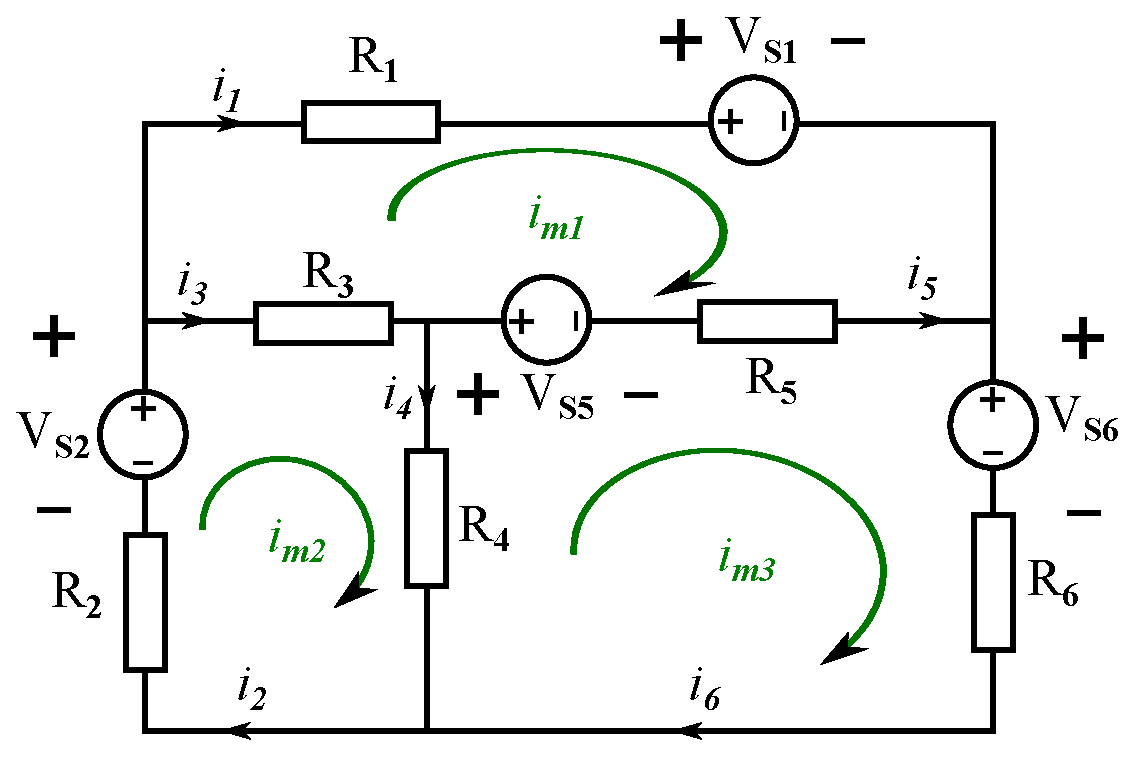
\includegraphics[width=0.45\textwidth]{./images/meshmethod}
\end{figure}

We first assume that the voltages drop of each branch are $u_1$ to $u_6$, and according to the Ohm`s law:

\begin{itemize} \itemsep1pt \parskip0pt \parsep0pt 
  \item[] \hspace{6.6 cm}\begin{equation}v_1 = R_1i_1 + V_{s1} = R_1i_{m1} + V_{s1}\end{equation}
  \item[] \hspace{6.6 cm}\begin{equation}v_2 = R_2i_2 - V_{s2} = R_2\end{equation}
  \item[] \hspace{6.6 cm}\begin{equation}v_3 = R_3i_3 = R_3(i_{m2} - i_{m1})\end{equation}
  \item[] \hspace{6.6 cm}\begin{equation}v_4 = R_4i_4 = R_4(i_{m2}-i_{m1})\end{equation}
  \item[] \hspace{6.6 cm}\begin{equation}v_5 = R_5i_5 + V_{s5} = R_5(i_{m3}-i_{m1}) + V_{s5}\end{equation}
  \item[] \hspace{6.6 cm}\begin{equation}v_6 = R_6i_6 + V_{s6}= R_6i_{m3} + V_{s6}\end{equation}
\end{itemize}










Apply KVL to mesh1, mesh2 and mesh3:

\begin{itemize} \itemsep1pt \parskip0pt \parsep0pt 
  \item[] \hspace{6.6 cm}\begin{equation}v_1 - v_3 - v_5 = 0\end{equation}
  \item[] \hspace{6.6 cm}\begin{equation}v_2 + v_3 + v_4 = 0\end{equation}
  \item[] \hspace{6.6 cm}\begin{equation}-v_4 + v_5 + v_6 = 0\end{equation}
\end{itemize}


By combining Eqs. (5.16) -- (5.24) we obtain :

\begin{itemize} \itemsep1pt \parskip0pt \parsep0pt 
  \item[] \hspace{6.6 cm}\begin{equation}(R_1 + R_3 + R_5)i_{m1} - R_3i_{m2} - R_5i_{m3} = V_{s5} - V_{s1}\end{equation}
  \item[] \hspace{6.6 cm}\begin{equation}-R_3i_{m1} + (R_2 + R_3 +R_4)i_{m2} - R_4i_{m3} = V_{s2}\end{equation}
  \item[] \hspace{6.6 cm}\begin{equation}-R_5i_{m1} - R_4i_{m2} + (R_4 + R_5 + R_6)i_{m3} = V_{s3}\end{equation}
\end{itemize}

If we assign \blue{\bf $R_1 = R_2 = R_6 =3\Omega$, $R_3 = 5\Omega$, $R_4 = 1\Omega$, $R_5 = 2\Omega$, $V_{s1} = 12V$, $V_{s2} = 10V$, $V_{s5} = 6V$, $V_{s6} = -20V$}


\begin{itemize} \itemsep1pt \parskip0pt \parsep0pt 
  \item[] \hspace{6.6 cm}\begin{equation}10i_{m1} - 5i_{m2} - 2i_{m3} = -6\end{equation}
  \item[] \hspace{6.6 cm}\begin{equation}-5i_{m1} + 9i_{m2} - i_{m3} = 10\end{equation}
  \item[] \hspace{6.6 cm}\begin{equation}-2i_{m1} - i_{m2} + 6i_{m3} = 14\end{equation}
\end{itemize}

Solve the equations we will get:


\begin{itemize} \itemsep3pt \parskip0pt \parsep0pt 
  \item[] \hspace{6.6 cm}$i_{m1} = 1A$
  \item[] \hspace{6.6 cm}$i_{m2} = 2A$
  \item[] \hspace{6.6 cm}$i_{m3} = 3A$
\end{itemize}

The current of each branch($i_1$ to $i_6$):


\begin{itemize} \itemsep3pt \parskip0pt \parsep0pt 
  \item[] \hspace{6.6 cm}$i_1 = i_{m1} = 1A$
  \item[] \hspace{6.6 cm}$i_2 = i_{m2} = 2A$
  \item[] \hspace{6.6 cm}$i_3 = i_{m2} - i_{m1} = 2-1 = 1A$
  \item[] \hspace{6.6 cm}$i_4 = i_{m2} - i_{m3} = 2-3 = -1A$
  \item[] \hspace{6.6 cm}$i_5 = i_{m3} - i_{m1} = 3-1 = 2A$
  \item[] \hspace{6.6 cm}$i_6 = i_{m3} = 3A$
\end{itemize}


\subsection{Equivalent Resistance}
\subsubsection{Thevenin's Theorem}
Any combination of batteries and resistances with two terminals can be replaced by a single voltage source \blue{\bf e} and a single series resistor \blue{\bf r}. The value of \blue{\bf e} is the \red{open circuit} voltage at the terminals, and the value of \blue{\bf r} is \blue{\bf e} divided by the current with the terminals short circuited.

\subsubsection{$\Delta-Y$ and $Y-\Delta$ Conversions}
In many circuit applications, we encounter components connected together in one of two ways to form a three-terminal network: the ``Delta'', or $\Delta$ (also known as the ``pi'', or $\Pi$) configuration, and the “Y” (also known as the “T”) configuration.

It's possible to calculate the proper values of resistors necessary to form one kind of network($\Delta or Y$) that behaves identically to the other kind. That is, if we had two separate resistor networks, one is $\Delta$-shape and the other is Y-shape, each with its resistors hidden from view, with nothing but the three terminals (A, B, and C) exposed for testing, the resistors could be sized for the two networks so that there would be no way to electrically determine one network apart from the other. In other words, equivalent $\Delta$ and Y networks behave identically.
The equations used to convert one network to the other are

\begin{paracol}{2}
\begin{leftcolumn*}

\begin{figure}[!ht]
  \caption{Wye(Y) network}
  \centering
  \includegraphics[width=0.2\textwidth]{./images/equ_resis1}
\end{figure}

\hspace{1.5 cm}{To convert a Delta($\Delta$) to a Wye(Y)}
\begin{equation}
R_A = \frac{R_{AB}R_{AC}}{R_{AB} + R_{AC} + R_{BC}}
\end{equation}
\begin{equation}
R_B = \frac{R_{AB}R_{BC}}{R_{AB} + R_{AC} + R_{BC}}
\end{equation}
\begin{equation}
R_C = \frac{R_{AC}R_{BC}}{R_{AB} + R_{AC} + R_{BC}}
\end{equation}

\end{leftcolumn*}

\begin{rightcolumn}

\begin{figure}[!ht]
  \caption{Delta($\Delta$) network}
  \centering
  \includegraphics[width=0.25\textwidth]{./images/equ_resis2}
\end{figure}
\vspace{0.5 cm}
\hspace{1.5 cm}To convert a Wye(Y) to a Delta($\Delta$)
\begin{equation}
R_{AB} = \frac{R_AR_B + R_AR_C + R_BR_C}{R_C}
\end{equation}
\begin{equation}
R_{BC} = \frac{R_AR_B + R_AR_C + R_BR_C}{R_A}
\end{equation}
\begin{equation}
R_{AC} = \frac{R_AR_B + R_AR_C + R_BR_C}{R_B}
\end{equation}
\end{rightcolumn}
\end{paracol}


A prime application for $\Delta$-Y conversion is in the solution of unbalanced bridge circuits, such as the one below:

\begin{figure}[!ht]
  \caption{$\Delta$-Y conversion example}
  \centering
  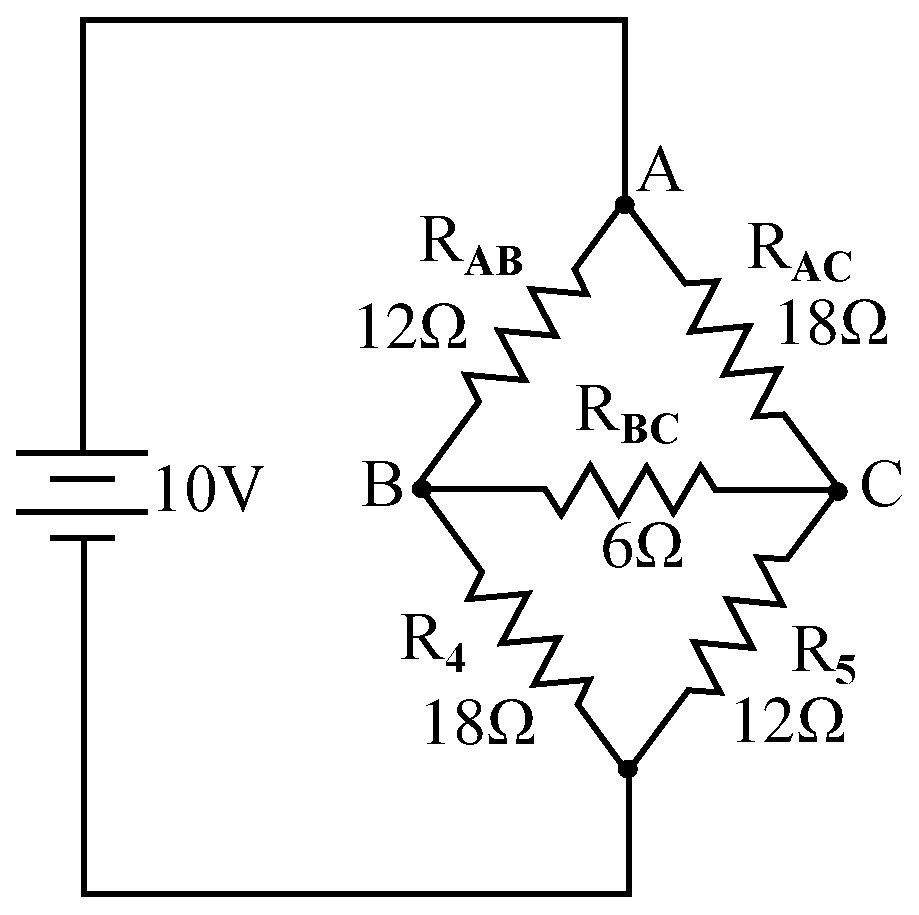
\includegraphics[width=0.25\textwidth,height=0.17\textheight]{./images/equ_resis3}
\end{figure}

Solution of this circuit with branch current or mesh current analysis is fairly involved, however methods like those are labor-consuming. If we were to treat resistors $R_{AB}$, $R_{AC}$, $R_{BC}$ as being connected in a $\Delta$ configuration and generate an equivalent Y network to replace them, we could turn this bridge circuit into a (simpler) series/parallel combination circuit:



\begin{figure}[!ht]
  \caption{After the $\Delta$-Y conversion}
  \centering
  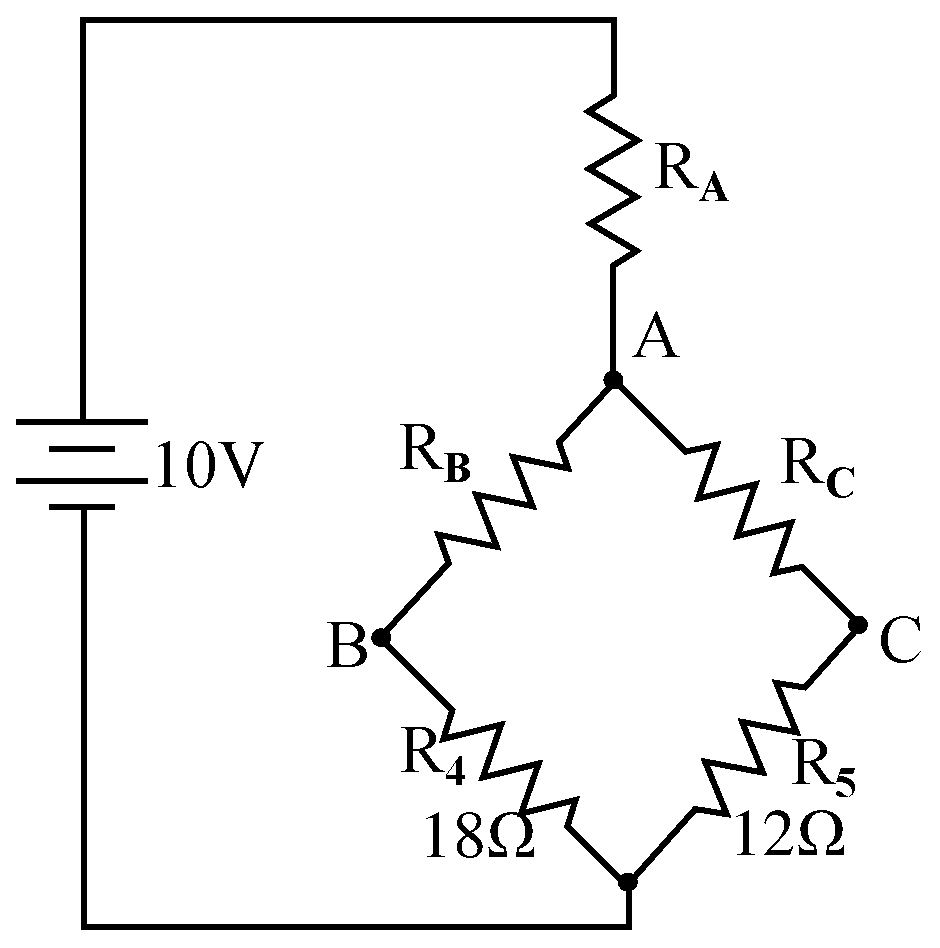
\includegraphics[width=0.25\textwidth,height=0.17\textheight]{./images/equ_resis4}
\end{figure}

If we perform our calculation correctly, the voltages between points $A$, $B$ and $C$ will be the same in the converted circuit as in the original circuit, and we can transfer those values back to the original bridge configuration.


\begin{equation}
R_{A} = \frac{(12\Omega)(18\Omega)}{(12\Omega)+(18\Omega)+(6\Omega)} = \frac{216}{36} = 6\Omega
\end{equation}
\begin{equation}
R_{B} = \frac{(12\Omega)(6\Omega)}{(12\Omega)+(18\Omega)+(6\Omega)} = \frac{72}{36} = 2\Omega
\end{equation}
\begin{equation}
R_{C} = \frac{(18\Omega)(6\Omega)}{(12\Omega)+(18\Omega)+(6\Omega)} = \frac{108}{36} = 3\Omega
\end{equation}
Resistors $R_4$ and $R_5$, of course, remain the same at $18\Omega$ and $12\Omega$, respectively. 


\subsubsection{Infinite Resistor Network}
Calculate the equivalent resistance of the following circuit combined with infinite resistors.

\begin{figure}[!ht]
  \caption{1-direction infinite ladder-shape resistor combination}
  \centering
  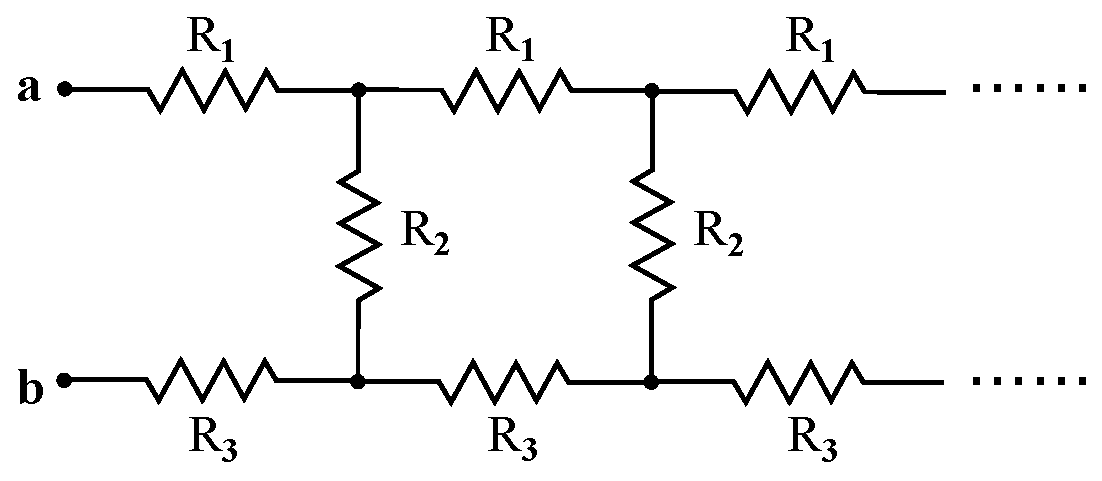
\includegraphics[width=0.5\textwidth]{./images/equ_resisinf1}
\end{figure}

\begin{itemize} \itemsep1pt \parskip0pt \parsep0pt 
  \item[\blue{\bf Analysis:}] The ladder-shape circuit above can be seen as composed with several {\bf``Part''} shown in Figure \ref{equ_resisinf1part}
\end{itemize}


\begin{figure}[!ht]
  \caption{Part}
  \label{equ_resisinf1part}
  \centering
  \includegraphics[width=0.2\textwidth]{./images/equ_resisinf1part}
\end{figure}

Since there are infinitely many resistors, there will still be infinitely many if we add(detach) another ``Part'' to the front section as shown in Figure \ref{equ_resisinf1comb}, and the resistance seen looking to the right between {\bf e} and {\bf f} will be the same as the resistance seen between {\bf a} and {\bf b}. That is $R_{ef} = R_{ab}$.

\begin{figure}[!ht]
  \caption{Add another ``part'' to the front}
  \label{equ_resisinf1comb}
  \centering
  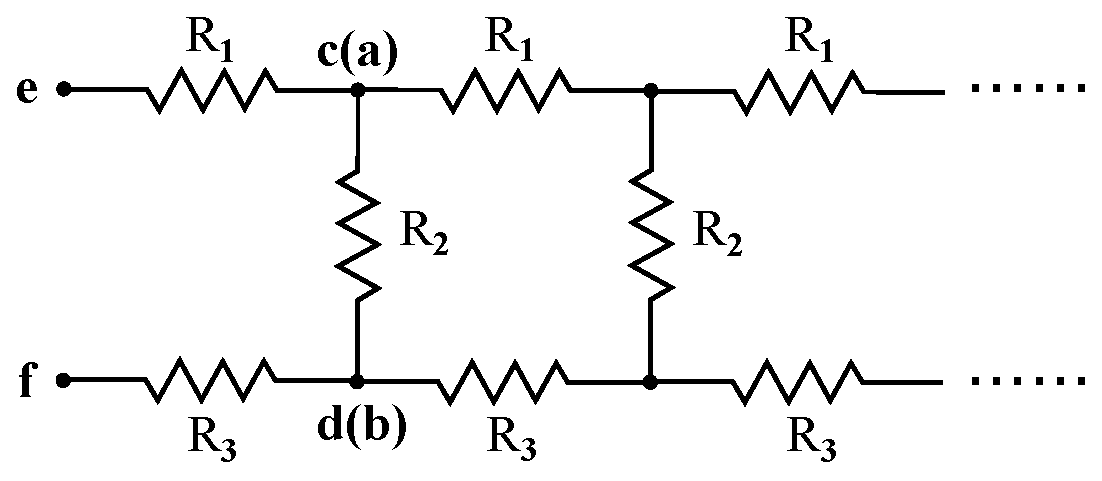
\includegraphics[width=0.5\textwidth]{./images/equ_resisinf1comb}
\end{figure}

From the Figure \ref{equ_resisinf1comb}, the equivalent resistance across {\bf e} and {\bf f} is:

\begin{itemize} \itemsep6pt \parskip0pt \parsep0pt
  \item[] \hspace{6 cm} $R_{ef} = R_1 + R_3 + R_{cd}(R_{ab})$
  \item[] \hspace{6 cm} $R_{ef} = R_1 + R_3 + (\frac{R_2R_{ab}}{R_2 + R_{ab}})$
\end{itemize}

Recall that \red{$R_{ef} = R_{ab}$}, so $R_{ab}$ can be expressed as:

\begin{equation}
R_{ab} = R_1 + R_3 + (\frac{R_2R_{ab}}{R_2 + R_{ab}})
\end{equation}

\begin{equation}
R_{ab} = \frac{R_1 + R_3 + \sqrt{(R_1 + R_3)(R_1 + R_3 + 4R_2)}}{2}
\end{equation}

Likewise, the following circuits have their equivalent resistances are shown as follow:

\begin{figure}[!ht]
  \caption{1-direction infinite ladder-shape2}
  \label{equ_resisinf1_1}
  \centering
  \includegraphics[width=0.5\textwidth]{./images/equ_resisinf1_1}
\end{figure}

\begin{equation}
R_{ab} = \frac{R_1 + R_3 + \sqrt{(R_1 + R_3)(R_1 + R_3 + 4R_2)}}{2}
\end{equation}

\begin{figure}[!ht]
  \caption{2-direction infinite ladder-shape1}
  \label{equ_resisinf2}
  \centering
  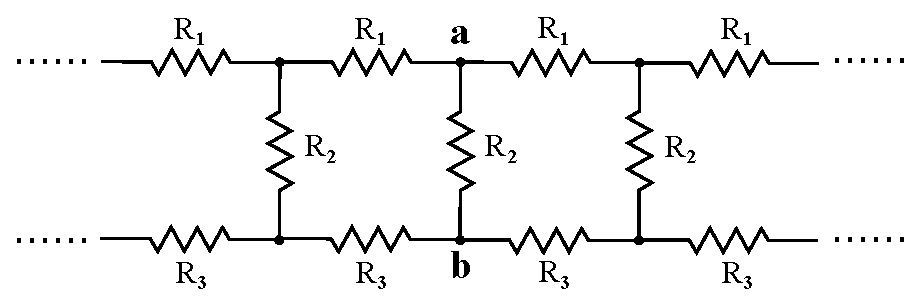
\includegraphics[width=0.5\textwidth]{./images/equ_resisinf2}
\end{figure}

\begin{equation}
R_{ab} = R_2\sqrt{\frac{(R_1 + R_3)}{(R_1 + R_3 + 4R_2)}}
\end{equation}
\vspace{3 cm}


\begin{figure}[!ht]
  \caption{2-direction infinite ladder-shape2}
  \label{equ_resisinf3}
  \centering
  \includegraphics[width=0.5\textwidth]{./images/equ_resisinf3}
\end{figure}

\begin{equation}
R_{ab} = \frac{R_1 + R_3 + \sqrt{(R_1 + R_3)(R_1 + R_3 + 4R_2)}}{4}
\end{equation}


\begin{figure}[ht]
  \caption{2-direction infinite ladder-shape3}
  \label{equ_resisinf4}
  \centering
  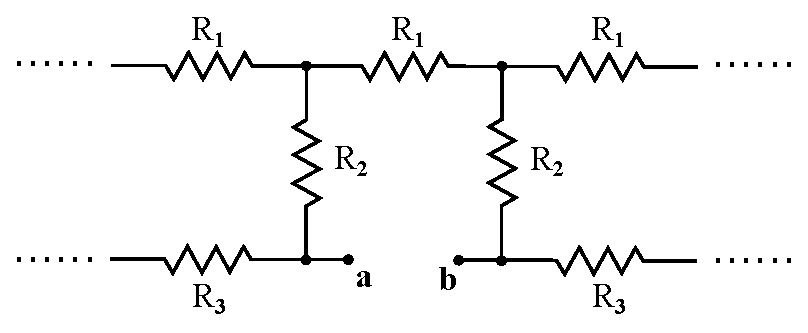
\includegraphics[width=0.5\textwidth]{./images/equ_resisinf4}
\end{figure}

\begin{equation}
R_{ab} = \sqrt{(R_1 + R_3)(R_1 + R_3 + 4R_2)}-R_3
\end{equation}



%
%
\end{document}
%%------------ Arman Shokrollahi--------------%%
